\begin{frame}
  \frametitle{Description of MSRE Pump Experiments}
  \begin{itemize}
    \item Starting from zero-power critical states under static/steady-flow conditions, the fuel salt pump
  was started up/coasted down.
    \item Reactor was kept critical by a flux-servo controller moving the rod in response to flux
      changes.
  \end{itemize}
  \begin{block}{\textbf{MSR Physics Phenomena Involved}}
    \begin{itemize}
      \item DNP drift under time-varying flow
      \item Loss of delayed neutrons due to out-of-core DNP decay
    \end{itemize}
  \end{block}
  \begin{columns}
    \column{5.5cm}
    \begin{figure}
      \centering
      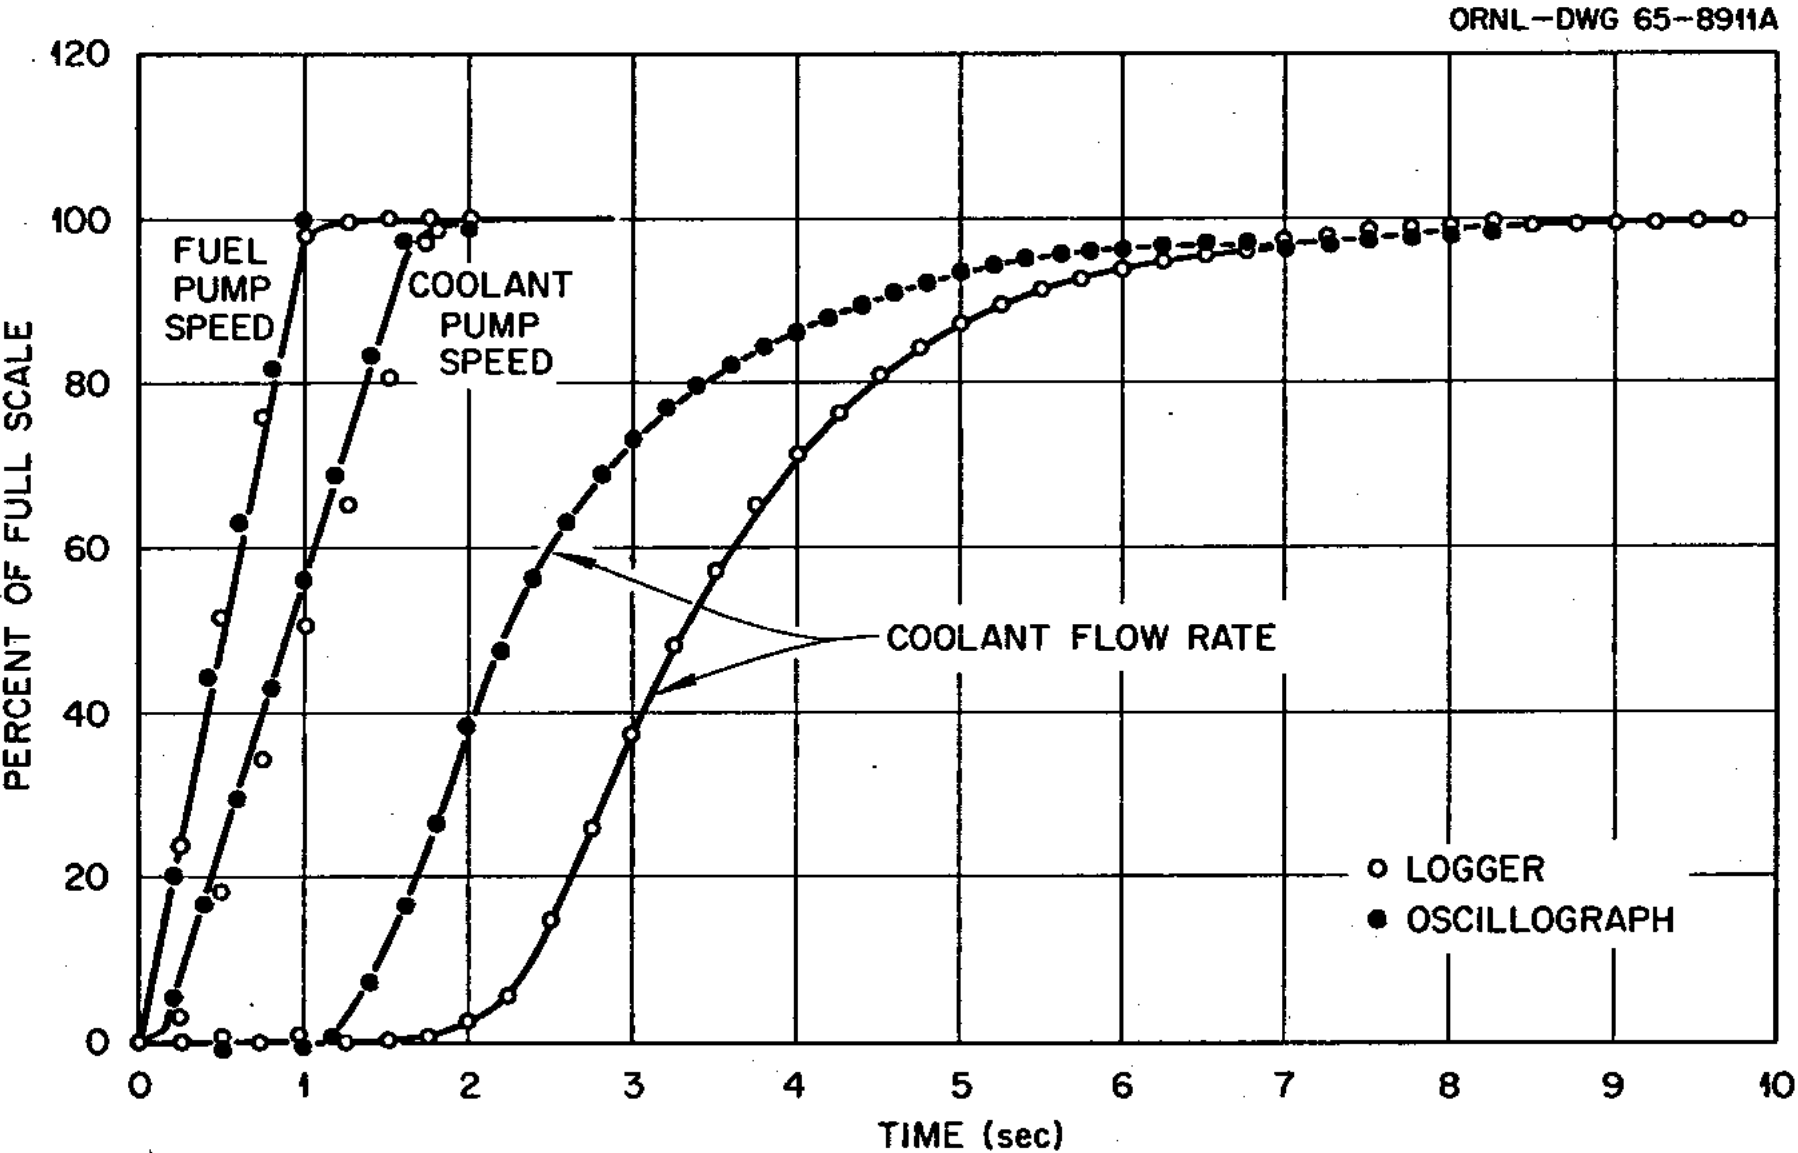
\includegraphics[width=.8\columnwidth]{images/msre-startup}
      \caption{MSRE start-up pump speed and flow rate experimental data
      \cite{prince_zero-power_1968}.}
    \end{figure}
    \column{5.5cm}
    \begin{figure}
      \centering
      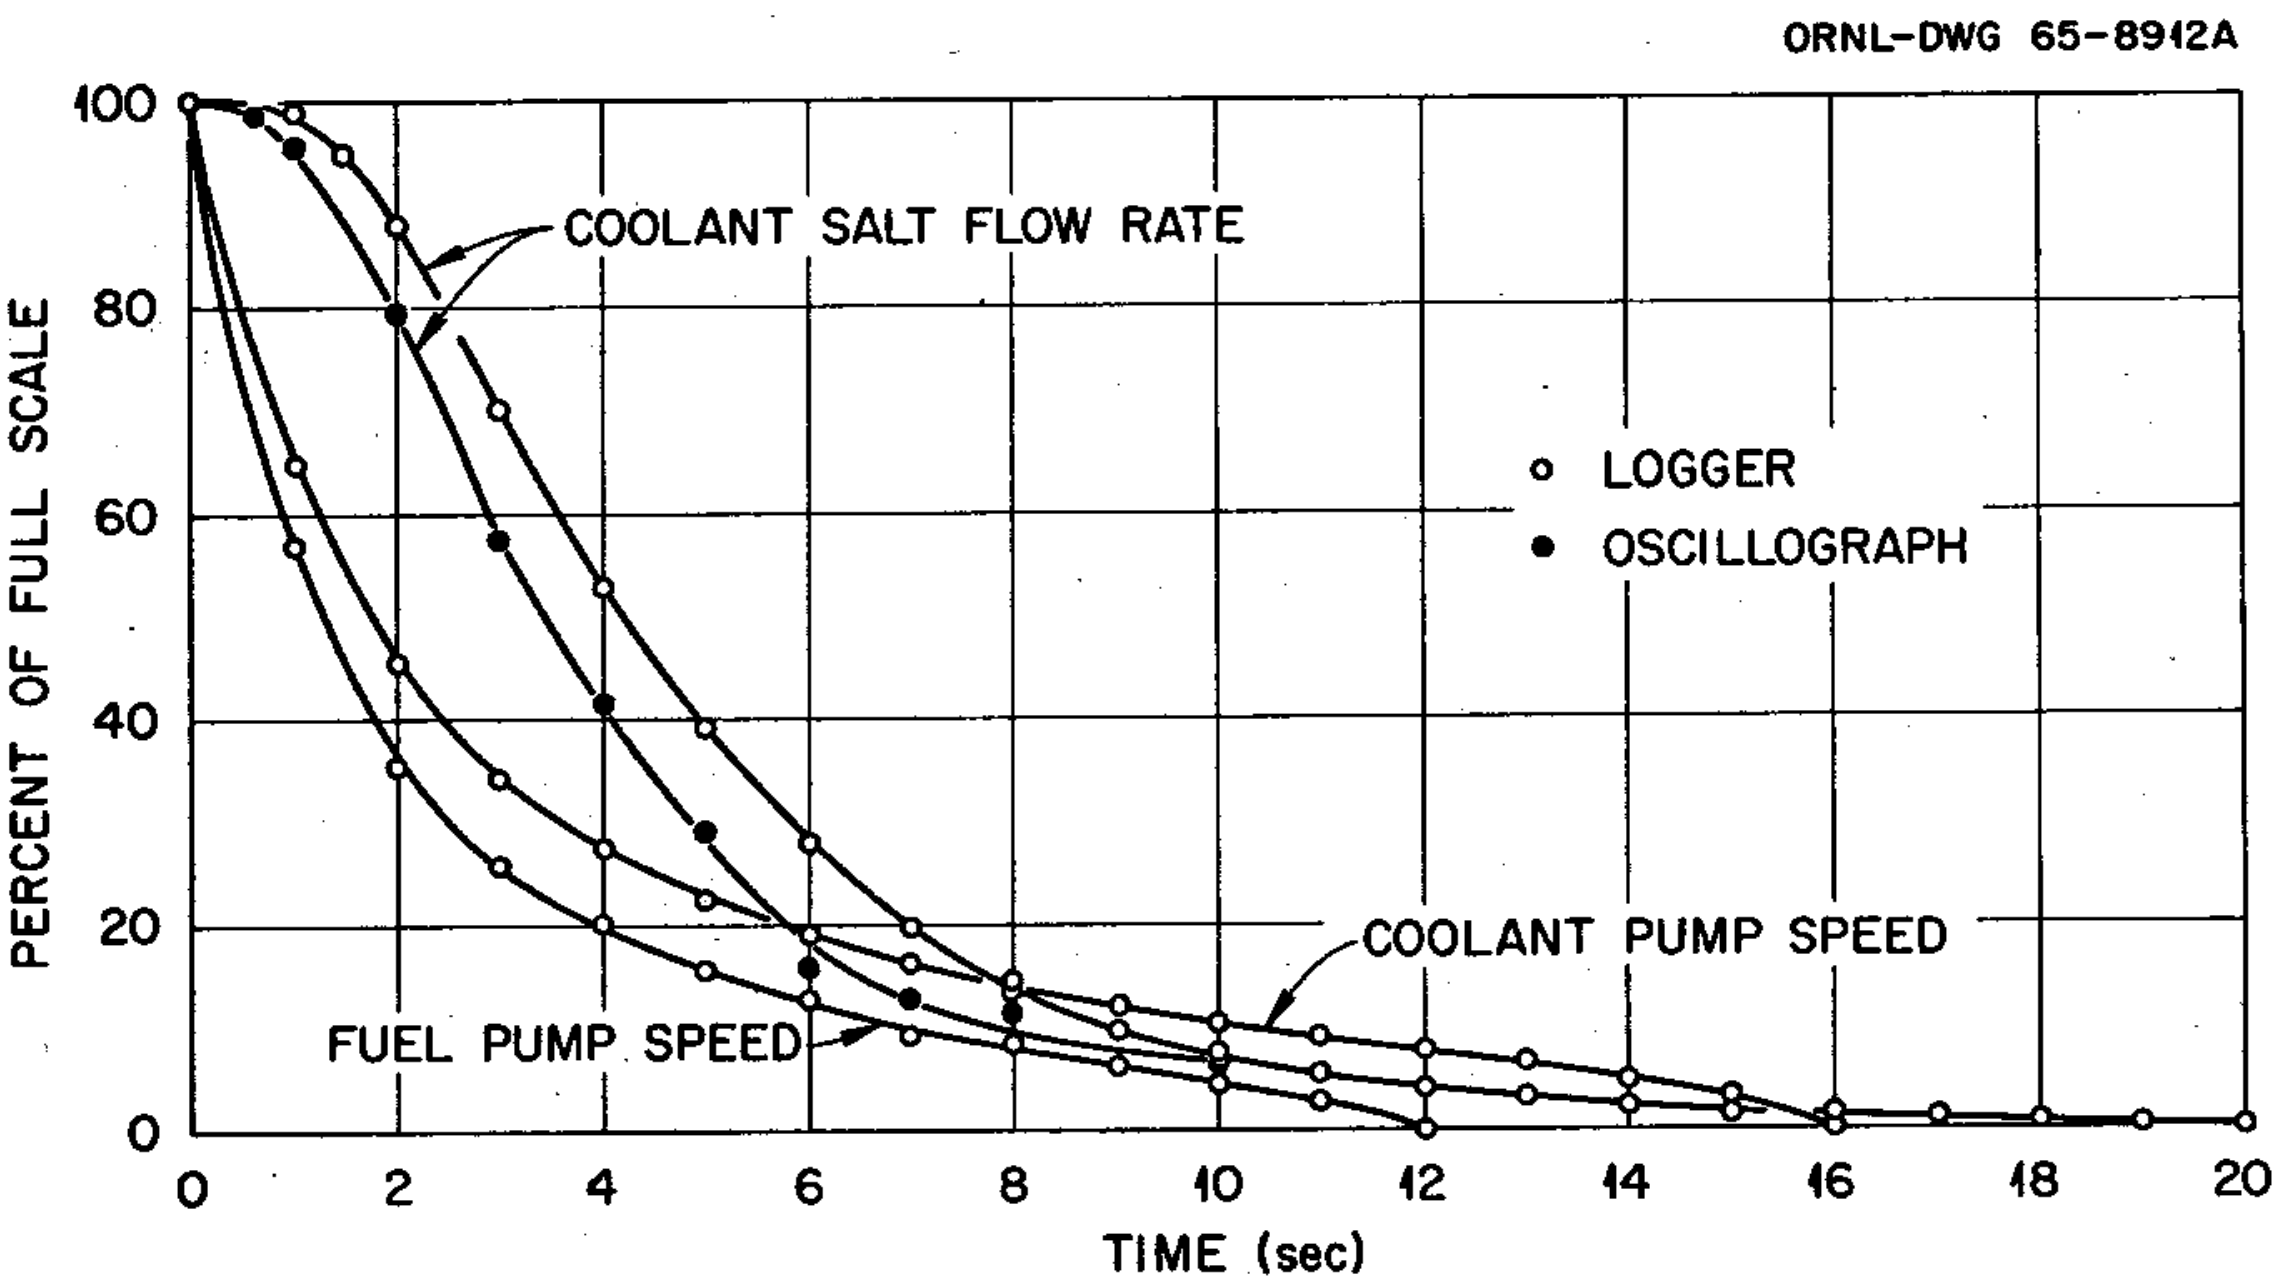
\includegraphics[width=.95\columnwidth]{images/msre-coastdown}
      \caption{MSRE coast-down pump speed and flow rate experimental data
      \cite{prince_zero-power_1968}.}
    \end{figure}
  \end{columns}
\end{frame}

%\begin{frame}
%  \frametitle{V\&V Study 2: MSRE Pump Start-up \& Coast-Down Transients}
%  \begin{block}{\textbf{MSR Phenomena Involved}}
%    \begin{itemize}
%      \item DNP drift under time-varying flow
%      \item Loss of delayed neutrons due to out-of-core DNP decay
%    \end{itemize}
%  \end{block}
%  \begin{block}{\textbf{Aim of the Study}}
%    Reproduce the reactivity curve of the control rod response with a 2-D axisymmetric model of the
%    MSRE in Moltres.
%  \end{block}
%  \begin{block}{\textbf{Study Objectives}}
%    \begin{itemize}
%      \item Develop a V\&V study based on the MSRE pump start-up \& coast-down
%        transients that is easily reproducible
%      \item Verify Moltres against QuasiMolto in collaboration with Aaron Reynolds
%        (formerly at Oregon State University)
%      \item Validate Moltres against MSRE experimental data for modeling \gls{DNP} drift
%    \end{itemize}
%  \end{block}
%\end{frame}

\begin{frame}
  \frametitle{V\&V Study: MSRE Pump Start-up \& Coast-Down Transients}
  \begin{columns}
    \column{6.5cm}
    \begin{block}{\textbf{Aim of the Study}}
      \begin{itemize}
         \item Develop a verification and validation (V\&V) study based on the MSRE pump transients
         \item Verify Moltres against QuasiMolto \cite{reynolds_analysis_2023} in collaboration
           with Dr.\ Aaron Reynolds
         \item Validate Moltres against MSRE experimental data for modeling \gls{DNP} drift
       \end{itemize}
    \end{block}
    \begin{block}{\textbf{Modeling Approach}}
      \begin{itemize}
        \item Two neutron energy groups and six DNP groups
        \item Ignored upper and lower plena in the geometry
%        \item Looped salt flow with a salt circulation time of 25.2 s
        \item $k$-eigenvalue calculation at every time-step ($dt=0.1$ s) in place of reactivity control
      \end{itemize}
    \end{block}
    \column{4.5cm}
    \begin{figure}[htb]
      \centering
      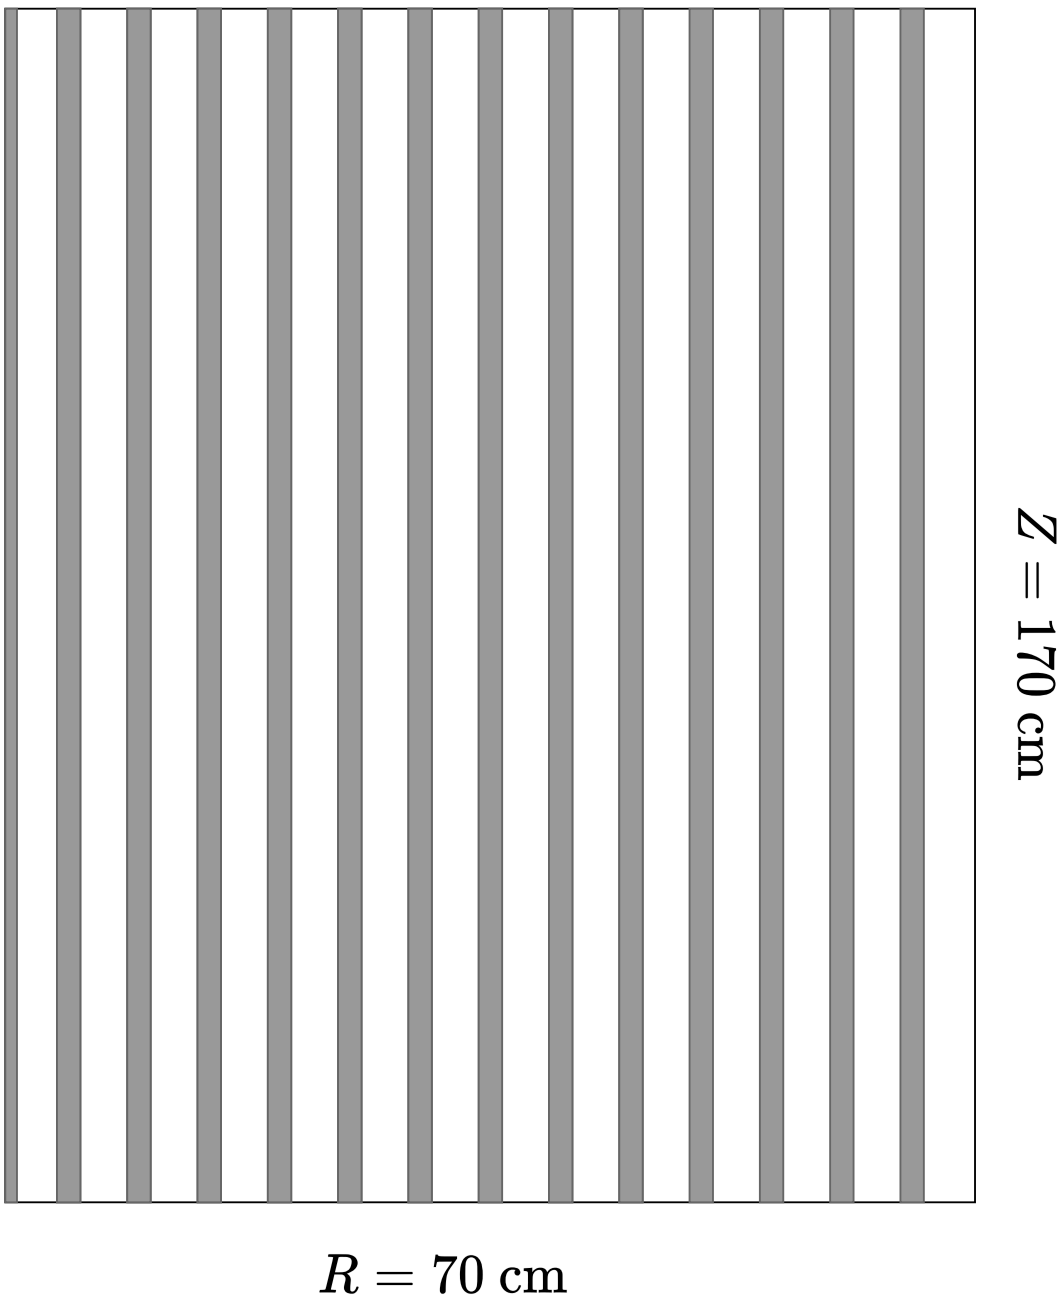
\includegraphics[width=0.8\columnwidth]{images/msre-2d}
      \caption{2-D axisymmetric model of the \gls{MSRE}.The gray and white regions represent fuel salt
      and graphite, respectively. Fuel salt channels are 1.25-cm wide and spaced at 5-cm intervals.}
      \label{fig:pump-geom}
    \end{figure}
  \end{columns}
\end{frame}

\begin{frame}
  \frametitle{MSRE $k_\text{eff}$ Estimates Under Static \& Steady-Flow Conditions}
  \begin{table}[htb]
    \centering
    \caption{Multiplication factors $k_\text{eff}$ under static and steady salt flow conditions, and
    reactivity changes $\Delta\rho$ due to \gls{DNP} flow from the Moltres and QuasiMolto \gls{MSRE}
    models.}
    \begin{tabular}{l S S S}
      \toprule
      \multirow{2}{*}{Code} & \multicolumn{2}{c}{$k_\text{eff}$} & {$\Delta\rho$ due to} \\
                            & {Static} & {Steady flow} & {\gls{DNP} flow} \\
                            \cmidrule(r){1-1} \cmidrule(rl){2-3} \cmidrule(l){4-4}
      Moltres & 1.05625 & 1.05311 & -282.4 \\
      QuasiMolto & 1.05603 & 1.05290 & -281.7 \\
      \bottomrule
    \end{tabular}
    \label{table:msre-pump-keff}
  \end{table}
  \begin{itemize}
    \item Excellent agreement between Moltres and QuasiMolto under static and steady-flow conditions prior
  to the pump transients.
  \end{itemize}
\end{frame}

\begin{frame}
  \frametitle{MSRE Neutron Flux Distributions Under Static Conditions}
  \begin{figure}[h]
    \centering
    \begin{subfigure}[b]{0.48\columnwidth}
      \centering
      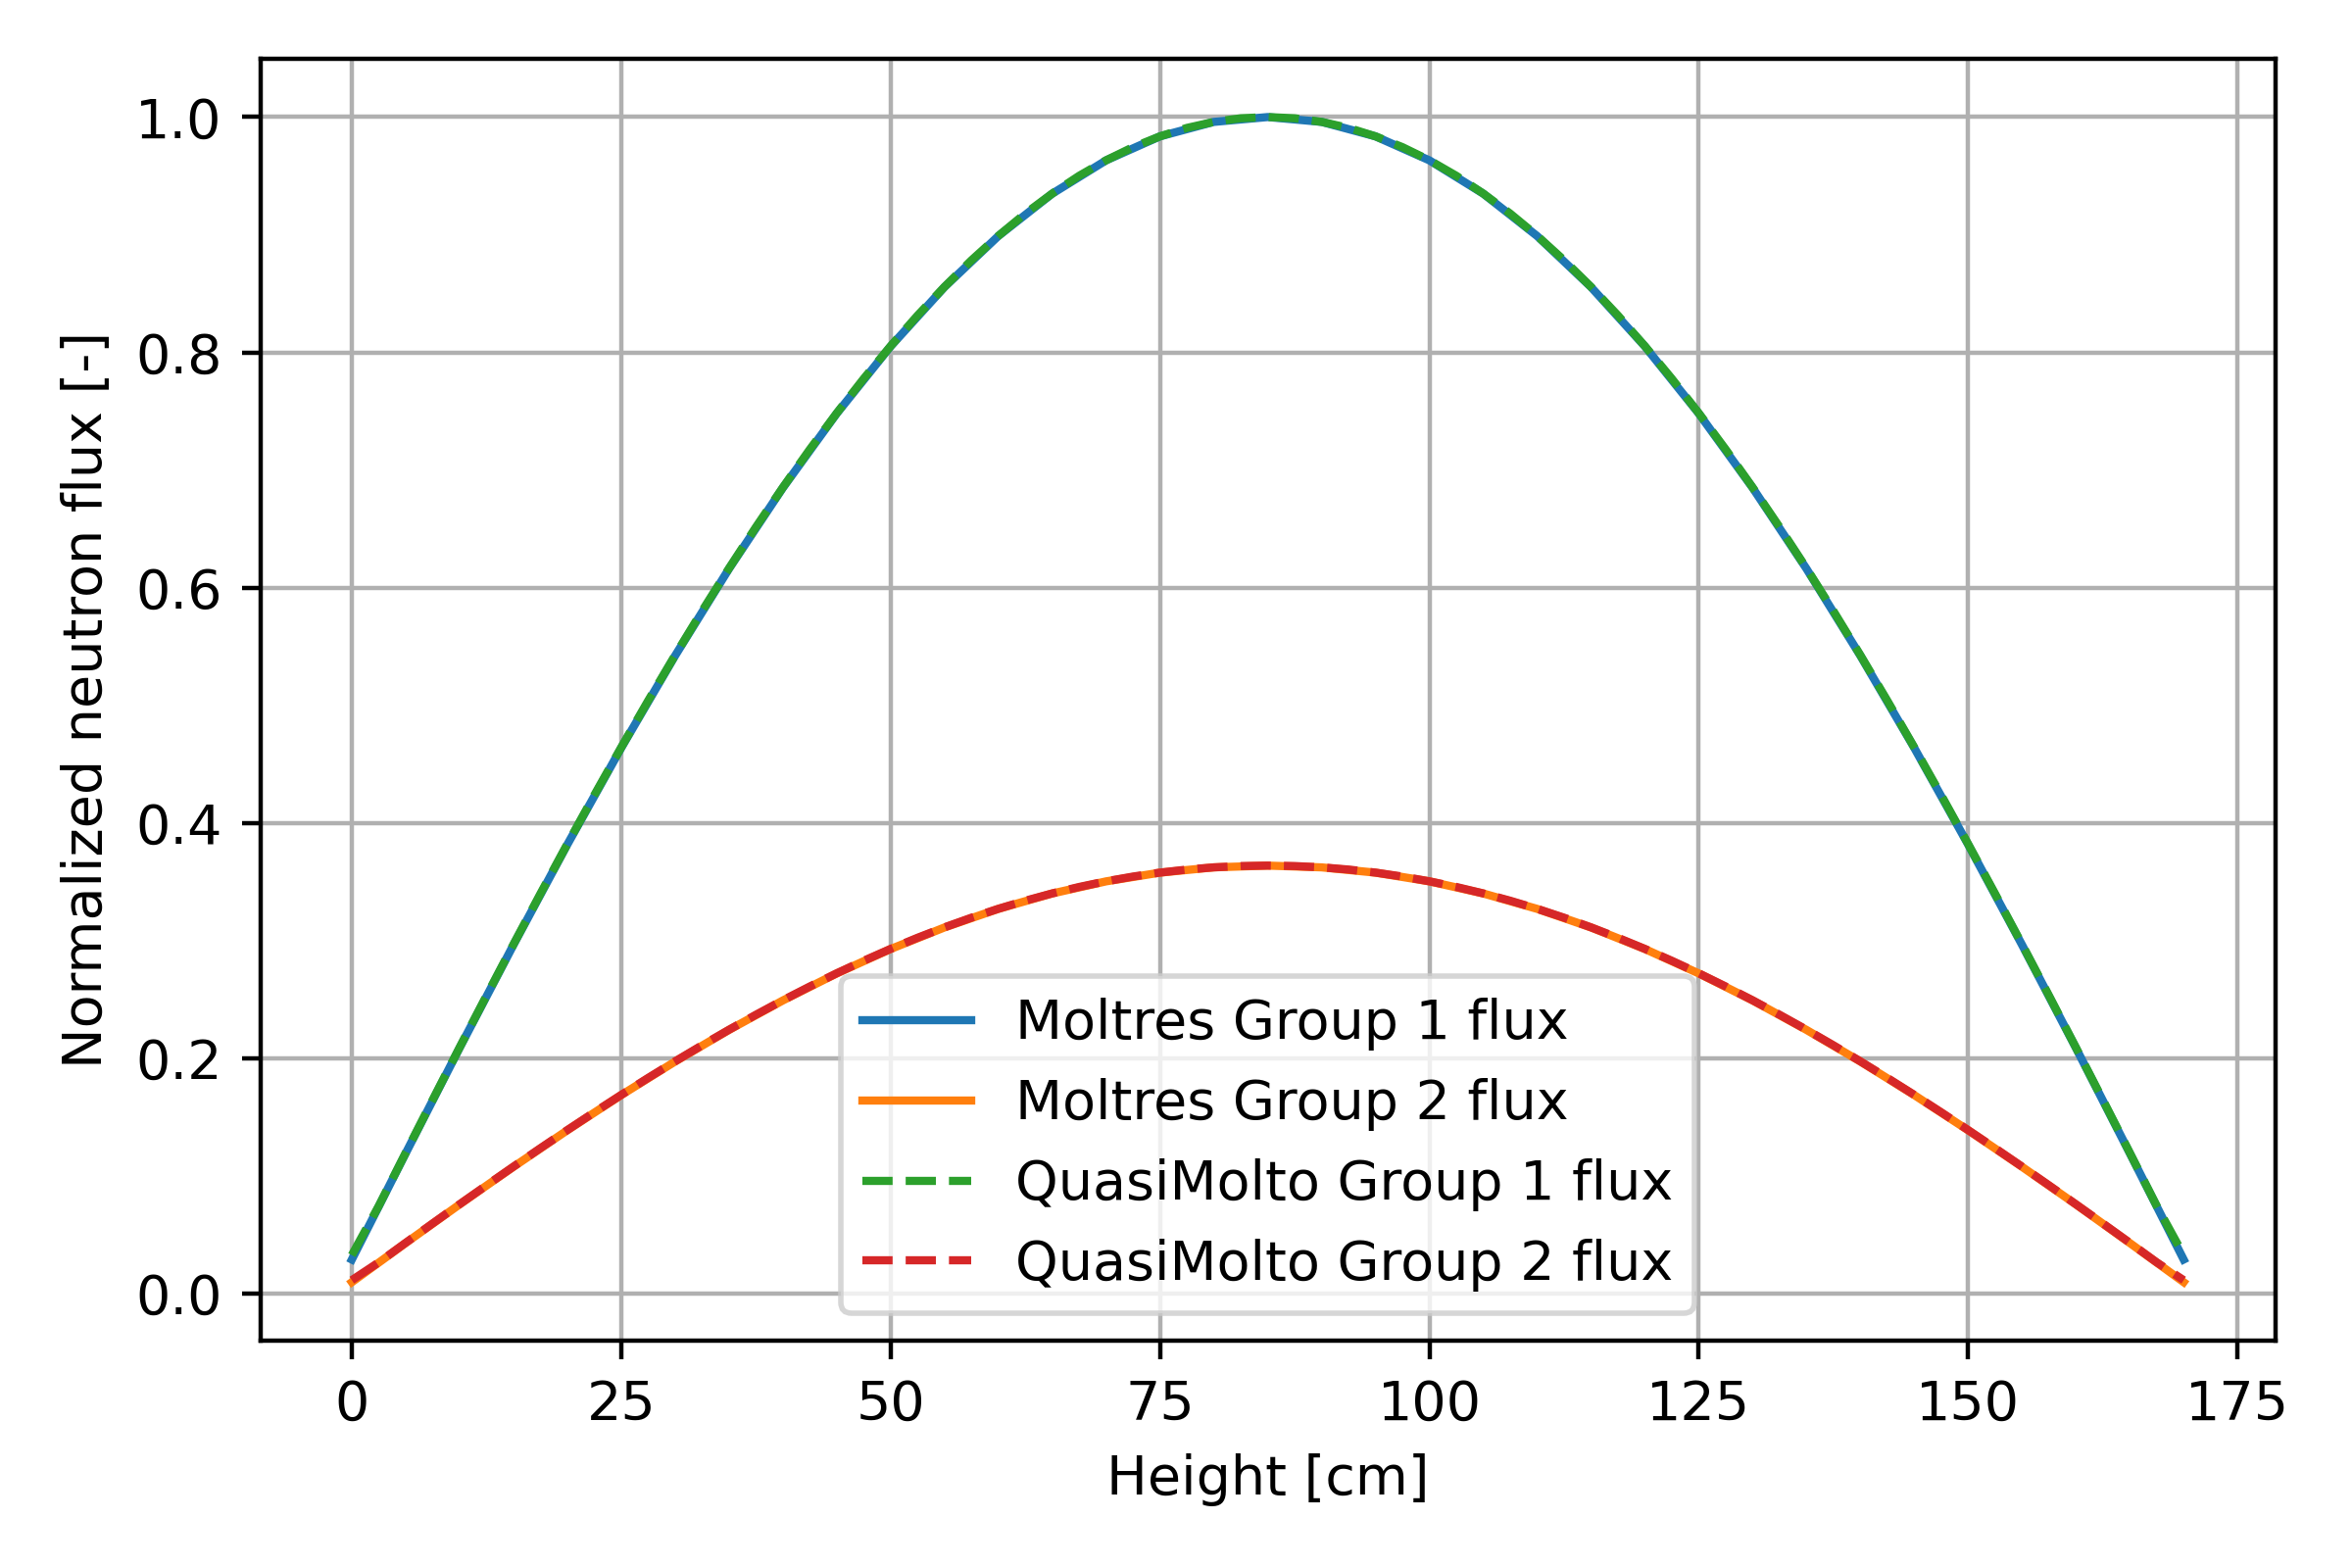
\includegraphics[width=\columnwidth]{centerline_flux}
      \caption{Normalized centerline neutron fluxes.}
      \label{fig:centerline-flux-dist}
    \end{subfigure}
    \hfill
    \begin{subfigure}[b]{0.48\columnwidth}
      \centering
      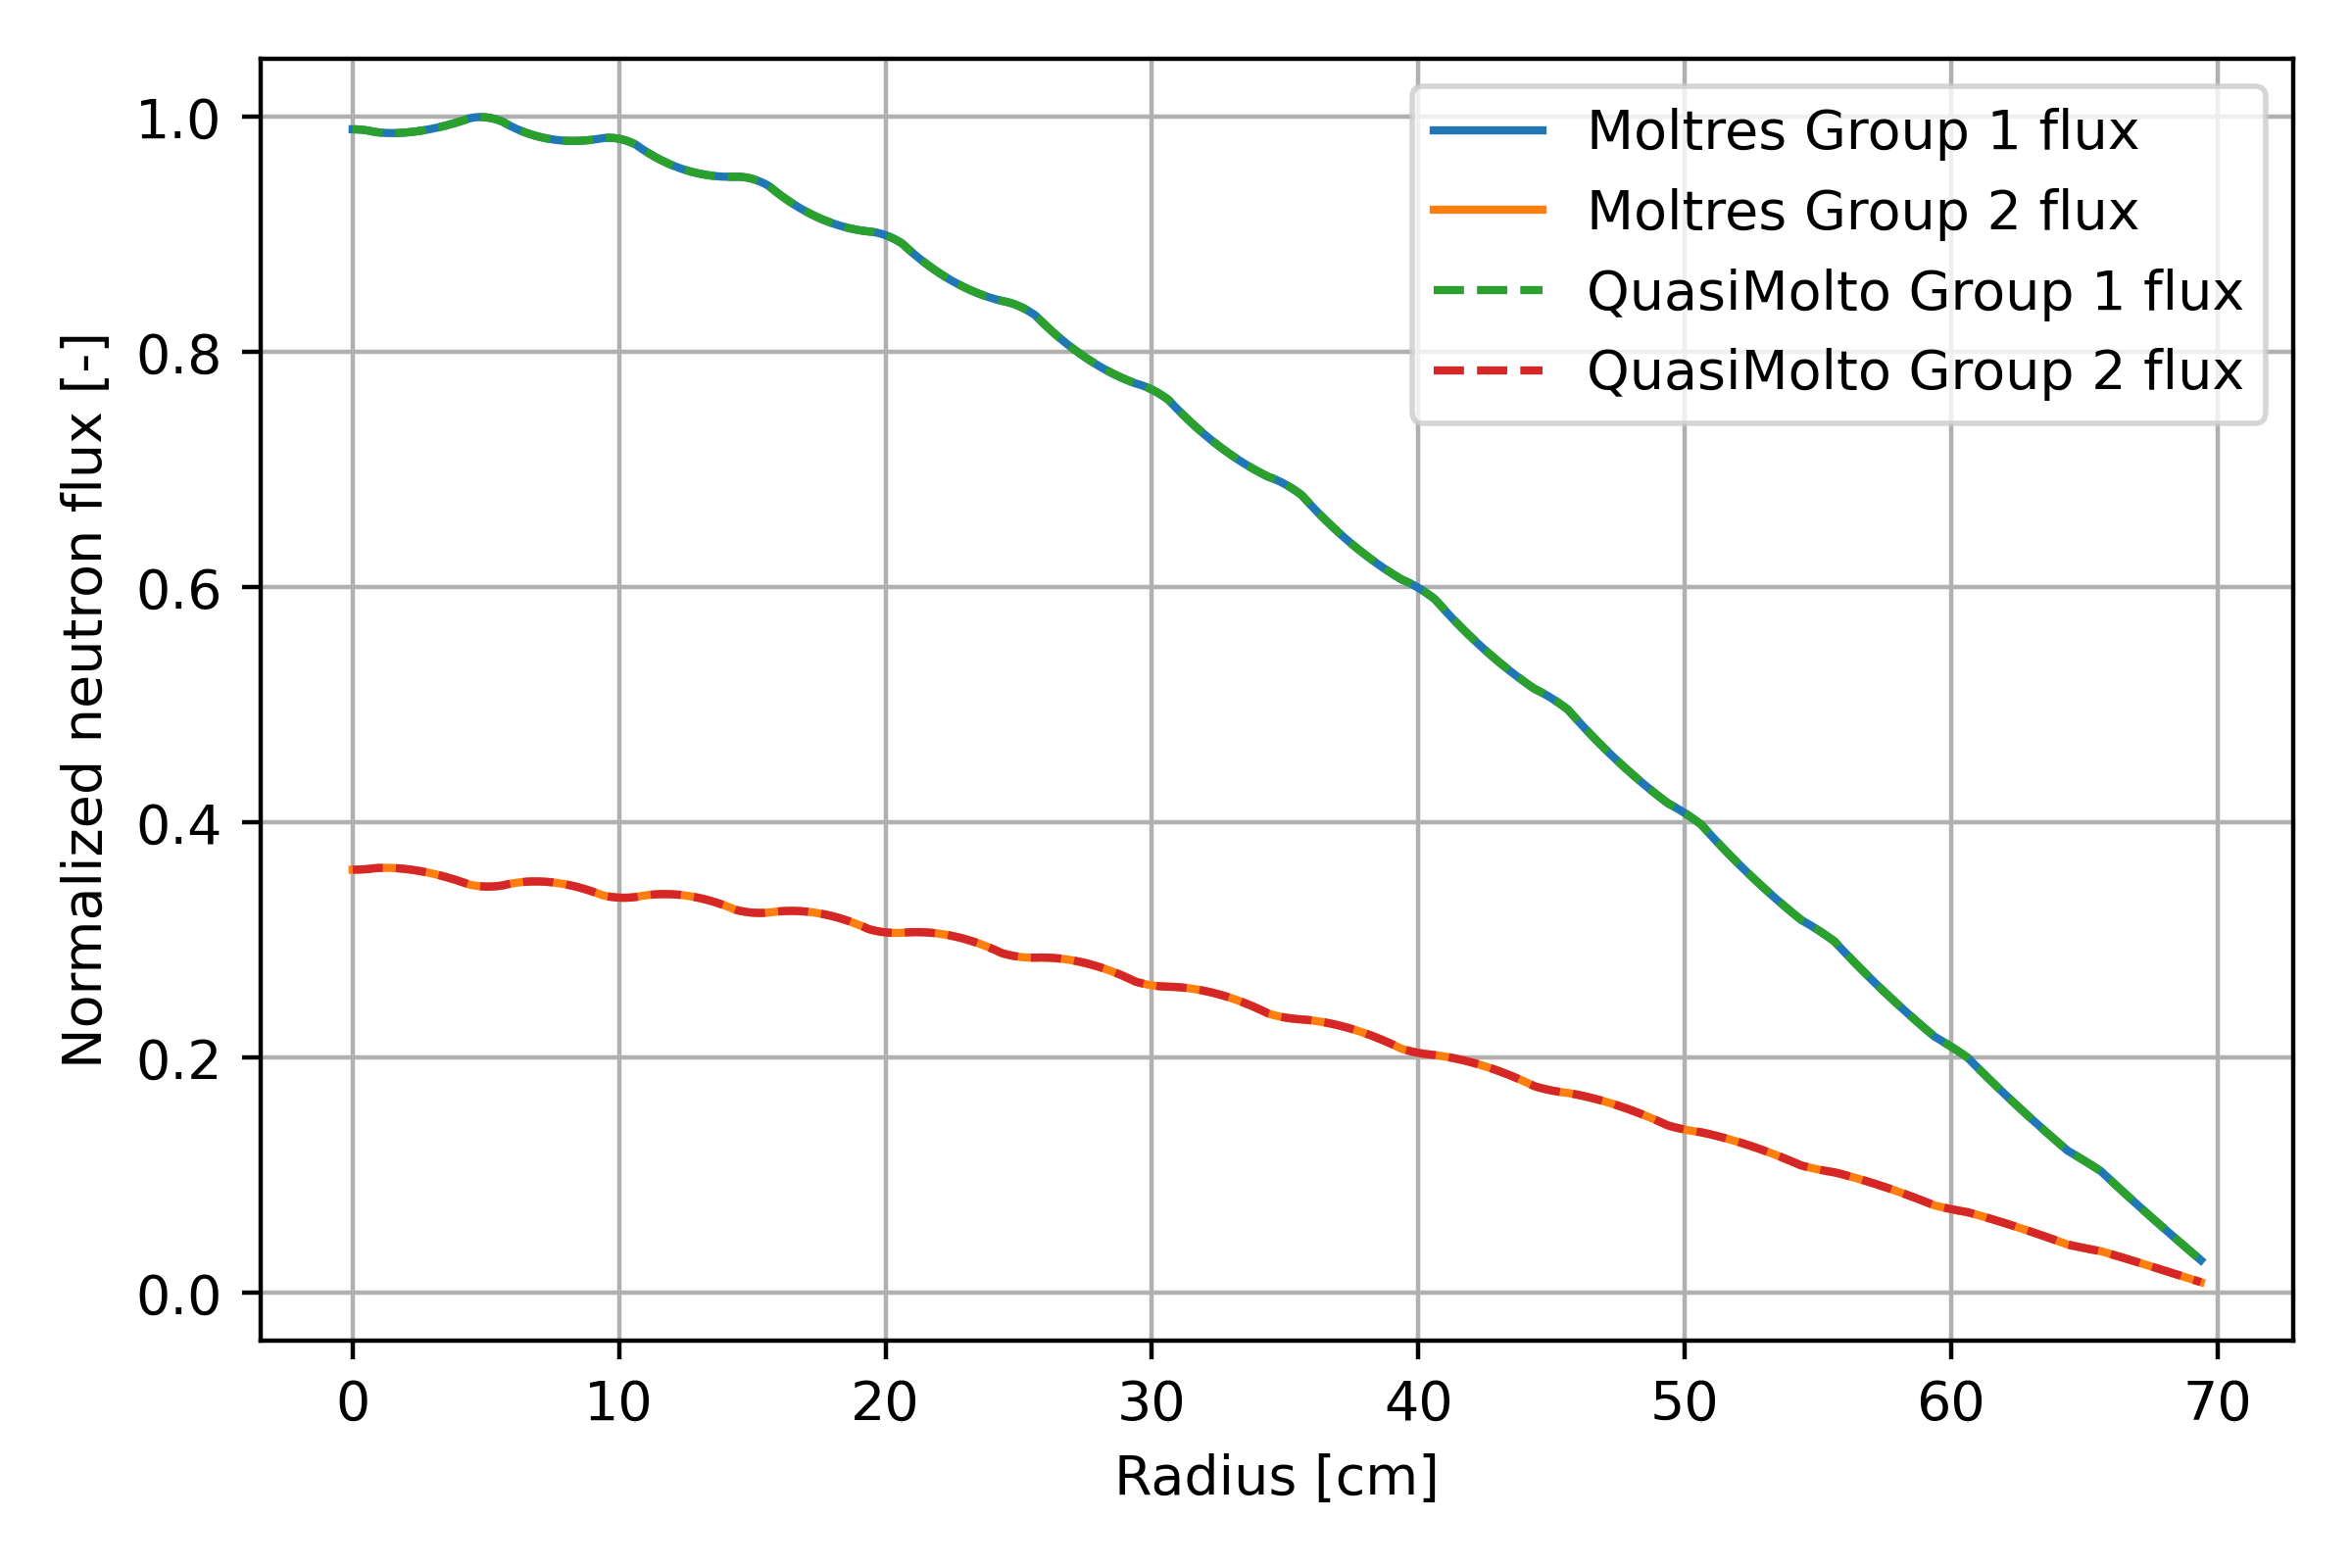
\includegraphics[width=\columnwidth]{midplane_flux}
      \caption{Normalized midplane neutron fluxes.}
      \label{fig:midplane-flux-dist}
    \end{subfigure}
    \caption{Neutron flux distributions comparing QuasiMolto and Moltres
    \gls{MSRE} models under static conditions. Maximum relative difference $\approx 0.8 \%$.}
    \label{fig:centerline-flux}
  \end{figure}
  \begin{itemize}
    \item Perfect overlap in centerline and midplane neutron fluxes between Moltres and QuasiMolto.
  \end{itemize}
\end{frame}

\begin{frame}
  \frametitle{MSRE Pump Start-Up Transient Results}
  \begin{columns}
  \column{5.5cm}
  \begin{figure}[t]
    \centering
    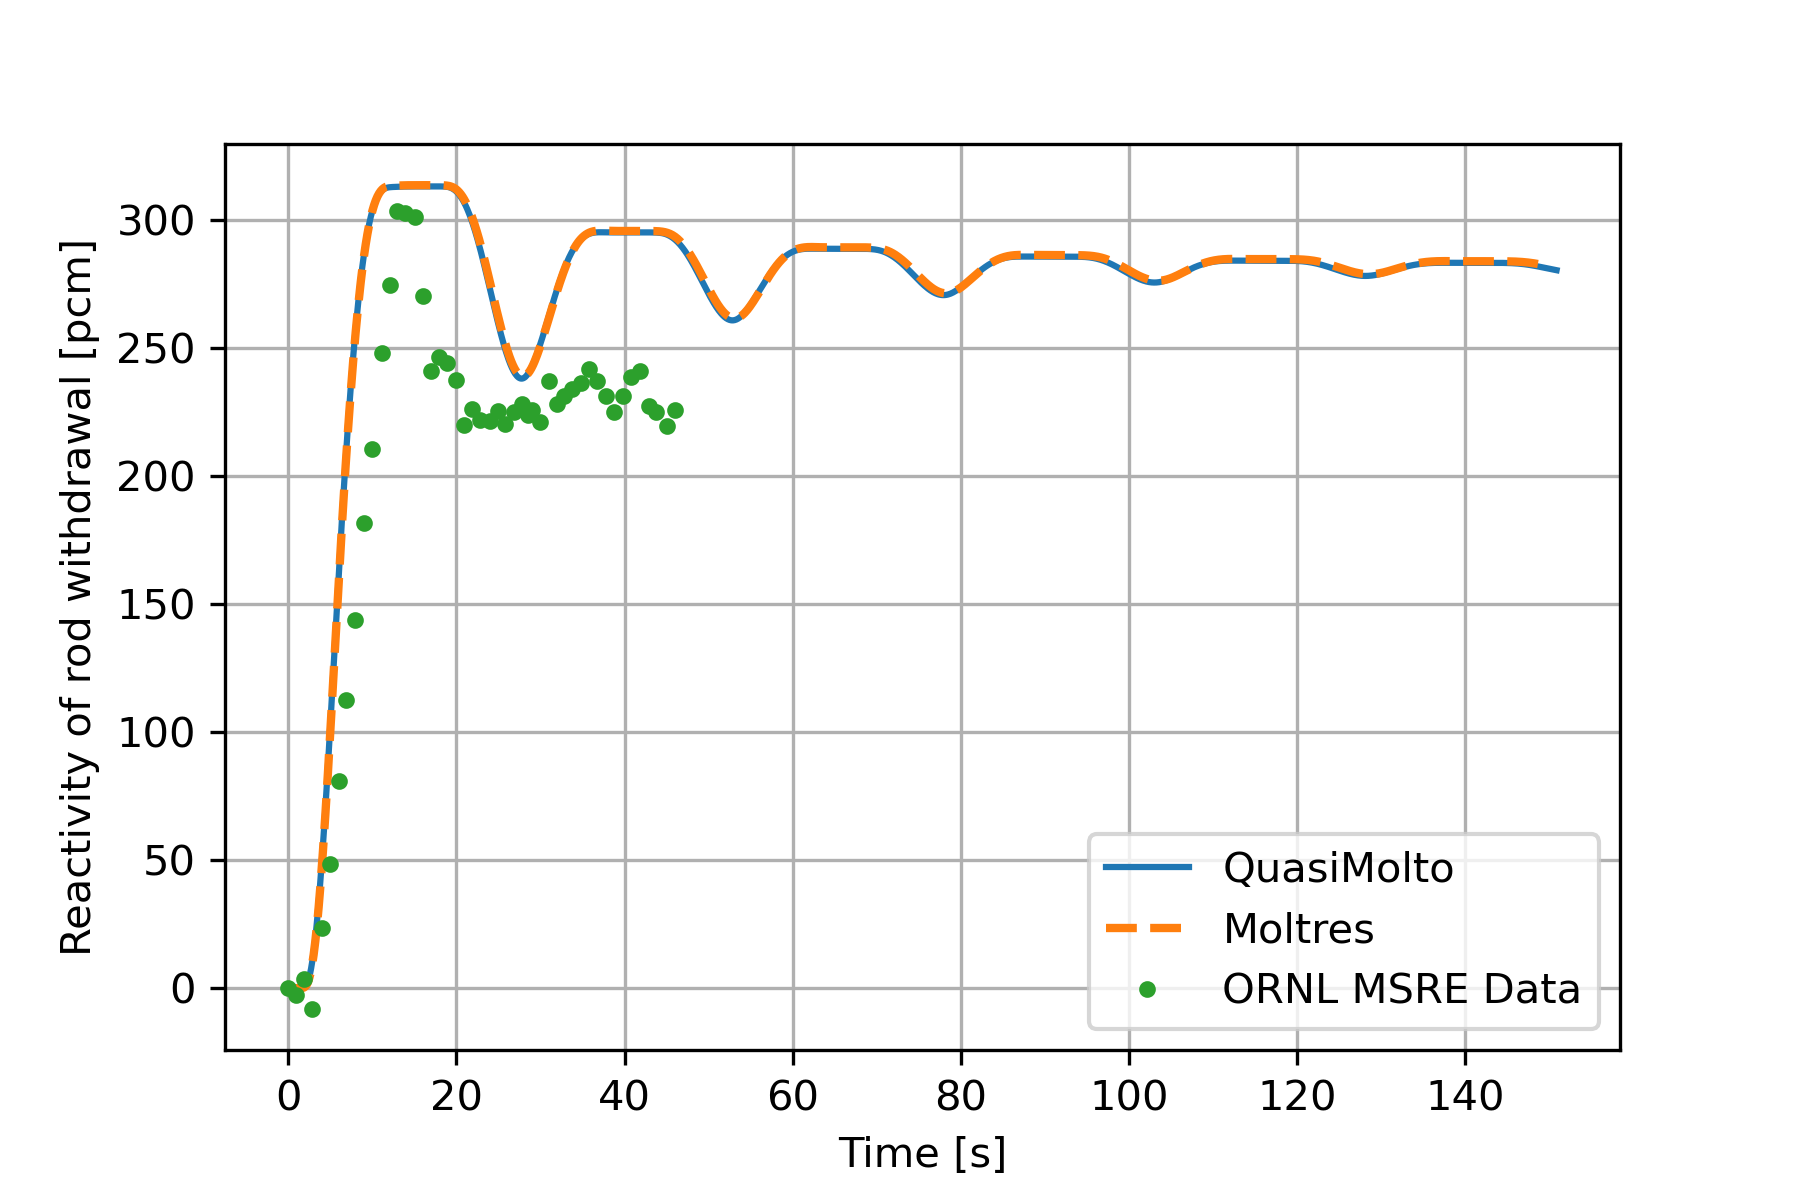
\includegraphics[width=\columnwidth]{start-up-v2-reactivity}
    \caption{Reactivity loss (relative to static conditions) during the \gls{MSRE} pump
    start-up transient.}
    \label{fig:start-up-reactivity}
  \end{figure}
  \column{5.5cm}
  \textbf{Numerical Results}
  \begin{itemize}
    \item Reactivity loss plateaus after excess DNPs exit.
    \item Circulation of the excess DNPs cause reactivity oscillations that eventually dissipate.
    \item Excellent agreement between Moltres and QuasiMolto.
  \end{itemize}
  \pause
  \textbf{Discrepancies against MSRE Data}
  \begin{itemize}
    \item MSRE had a smaller final reactivity loss.
    \item MSRE did not report a reactivity plateau (due to DNPs present in the upper and lower plena).
    \item MSRE did not log significant reactivity oscillations after the first peak.
  \end{itemize}
  \end{columns}
\end{frame}

%\begin{frame}
%  \frametitle{V\&V Study 2: MSRE Pump Start-up \& Coast-Down Transients}
%  \textbf{Pump Start-Up Transient Results}
%  \begin{columns}
%  \column{5.5cm}
%  \begin{figure}[t]
%    \centering
%    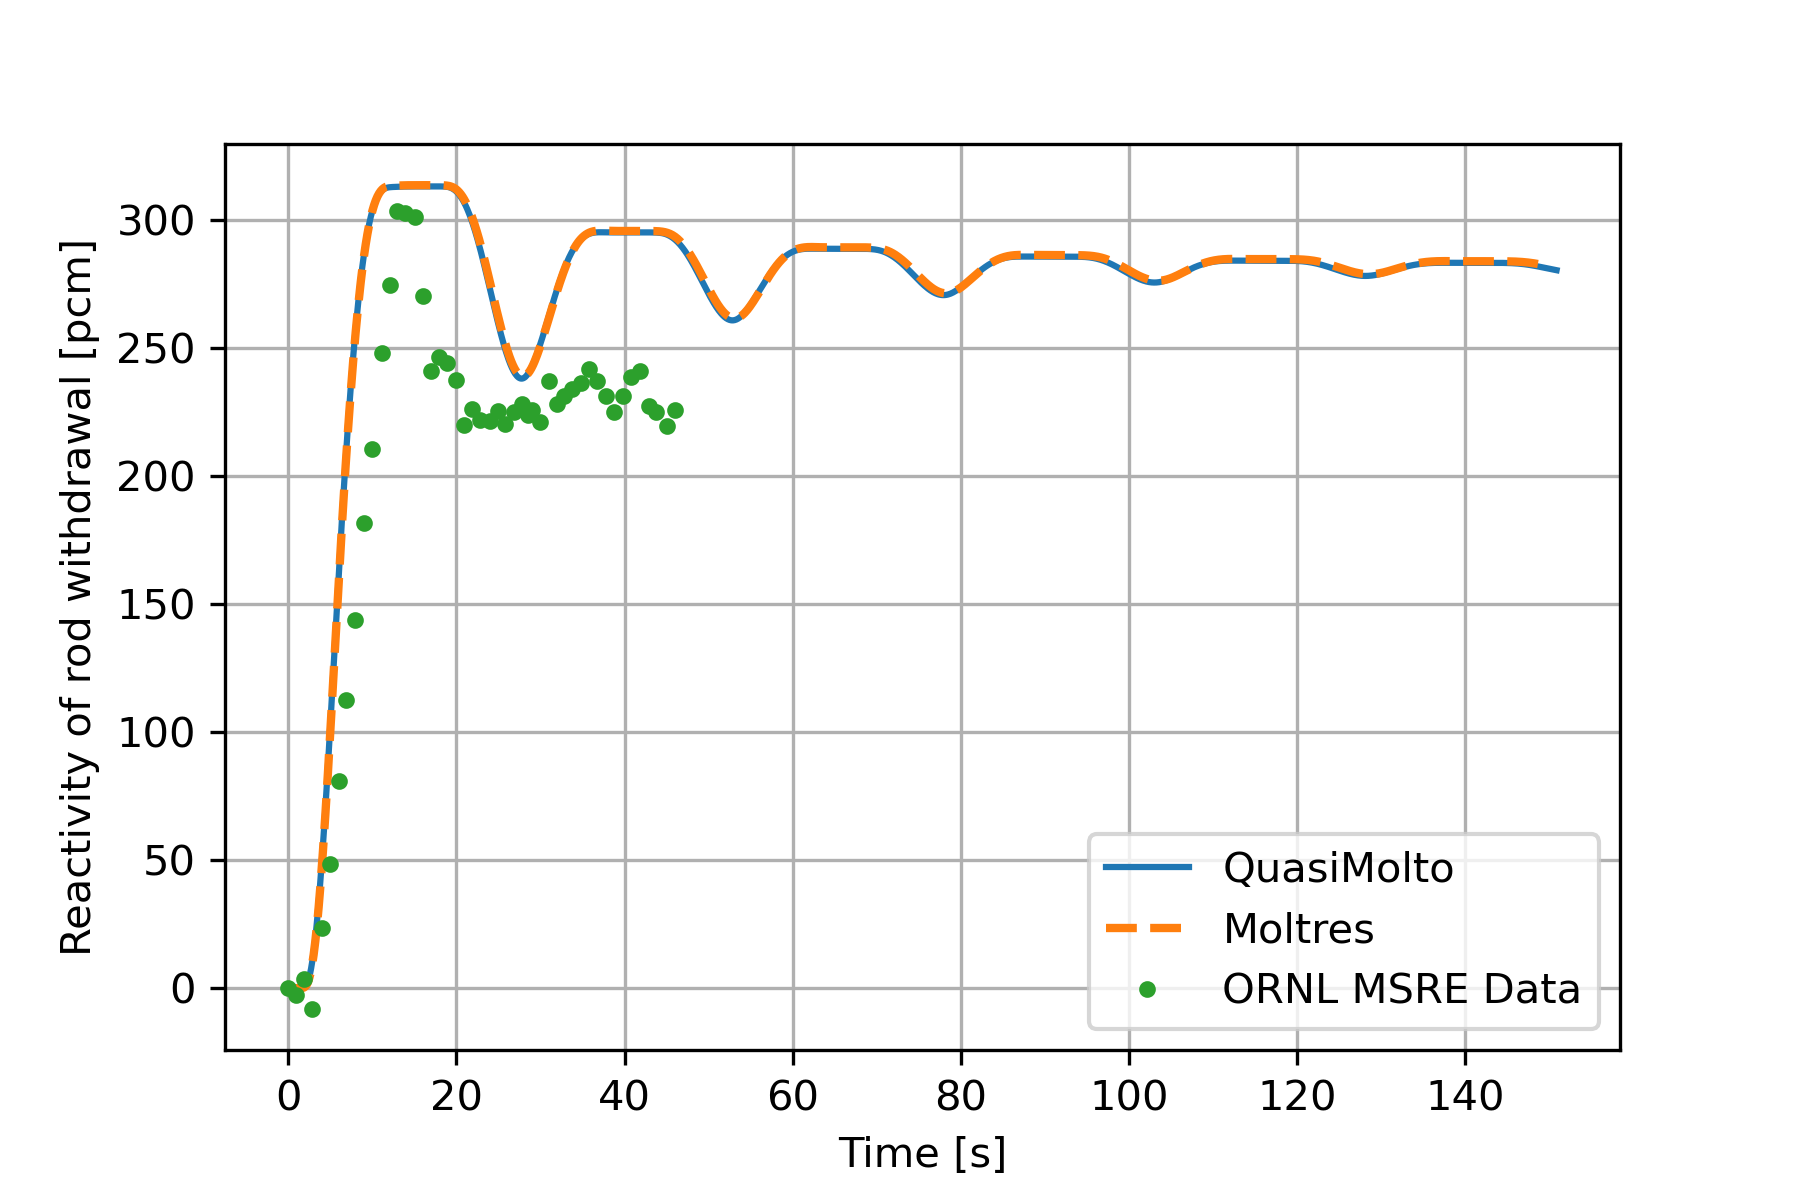
\includegraphics[width=\columnwidth]{start-up-v2-reactivity}
%    \caption{Reactivity loss (relative to static no-flow conditions) during the \gls{MSRE} pump
%    start-up transient.}
%    \label{fig:start-up-reactivity}
%  \end{figure}
%  \column{5.5cm}
%  \textbf{Discrepancies against MSRE Data}
%  \begin{itemize}
%    \item MSRE reported a smaller final reactivity loss
%    \item MSRE did not report a reactivity plateau (due to DNP present in the upper and lower plena)
%    \item MSRE did not log significant reactivity oscillations after the first peak
%  \end{itemize}
%  \end{columns}
%\end{frame}

\begin{frame}
  \frametitle{Pump Coast-Down Transient Results}
  \begin{figure}[t]
    \centering
    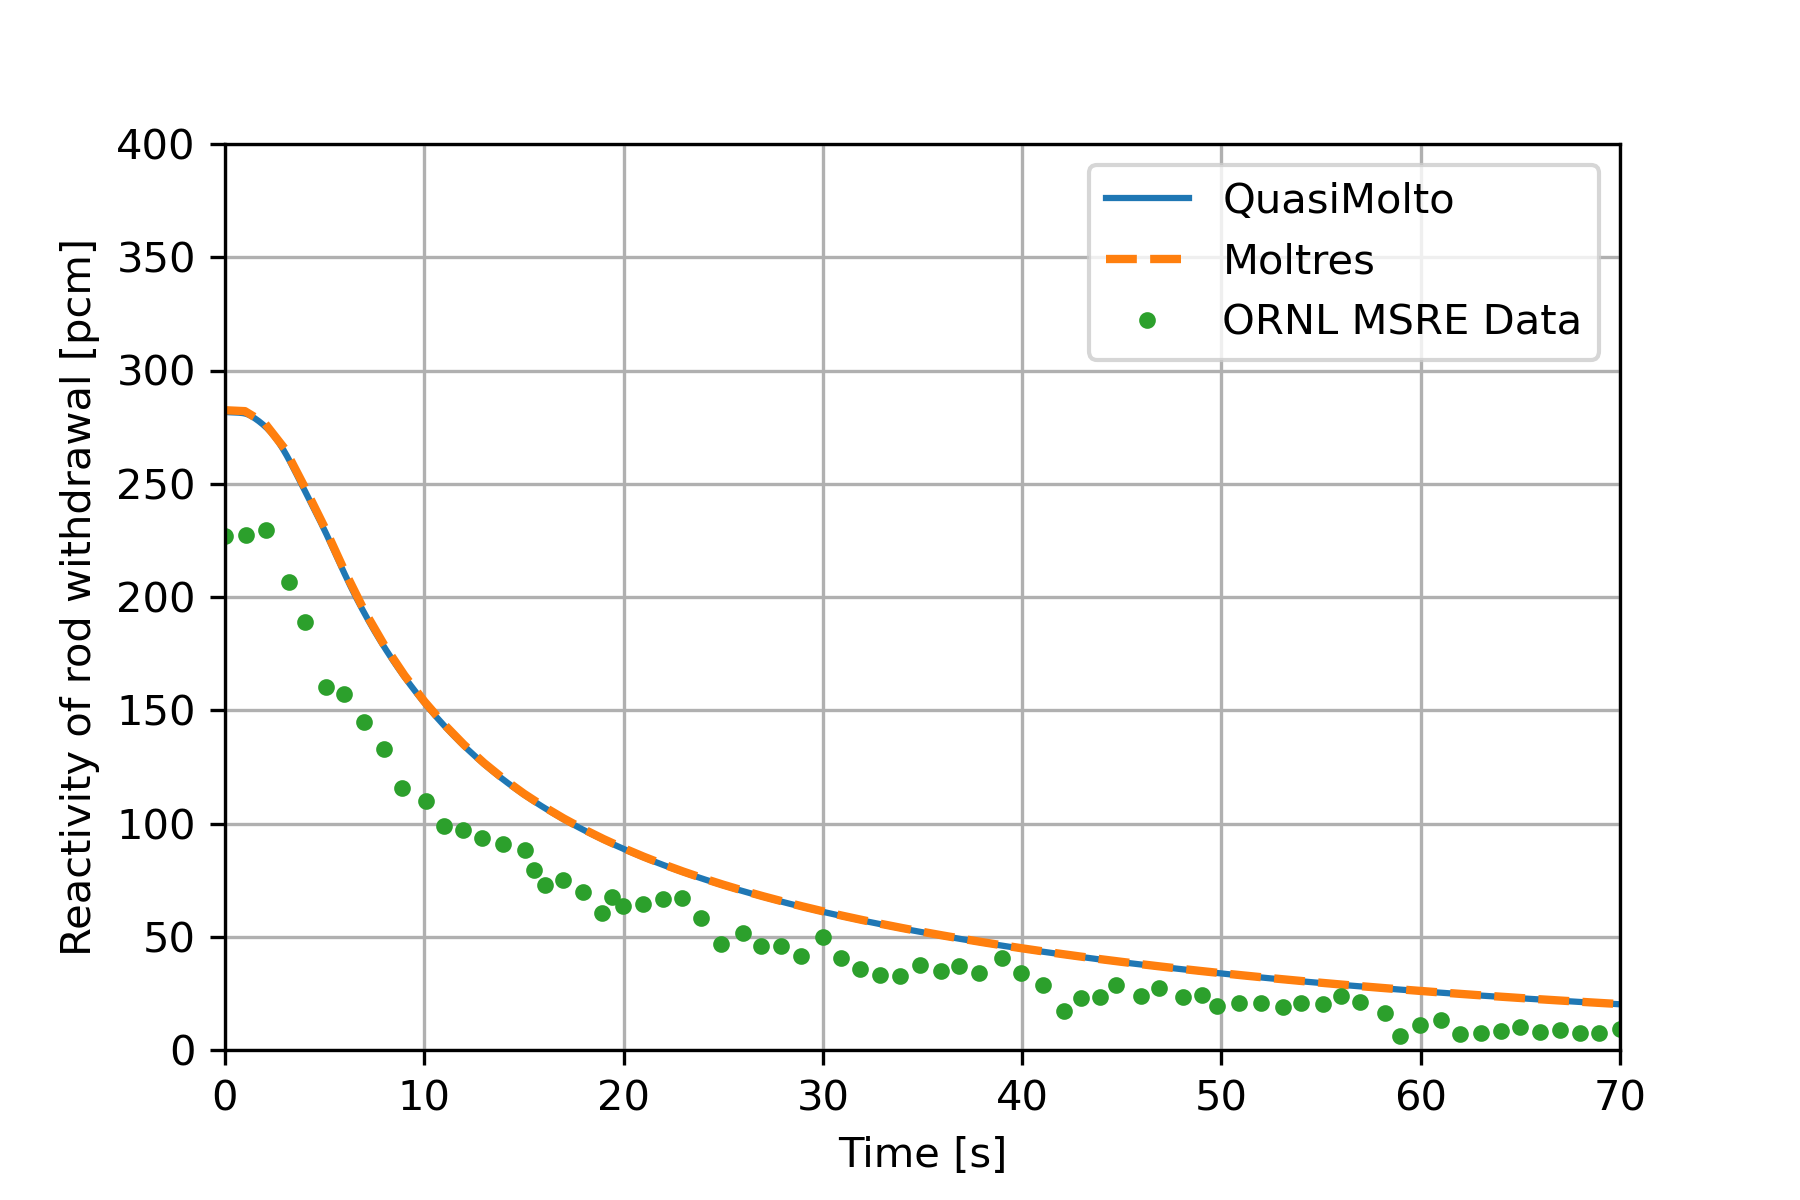
\includegraphics[width=.7\columnwidth]{coast-down-v2-reactivity}
    \caption{Reactivity loss (relative to static no-flow conditions) during the \gls{MSRE} pump
    coast-down transient.}
    \label{fig:start-up-reactivity}
  \end{figure}
  Good agreement between numerical and experimental data other than the magnitude differences.
\end{frame}

\begin{frame}
  \frametitle{Summary: MSRE Pump Start-up \& Coast-Down Transients}
  \begin{block}{\textbf{Study Outcome}}
    \begin{itemize}
      \item Moltres and QuasiMolto are highly consistent with each other in their looped DNP flow
        modeling capabilities
      \item Moltres and QuasiMolto reproduced key reactivity behavior in response to varying salt
        flow velocities
      \item Some discrepancies observed between the numerical and experimental results due to the
        omission of upper and lower plena
      \item This study can be used for verifying advection capabilities in other MSR simulation tools
      \item The distinct oscillations serve as valuable reference points to facilitate code-to-code
        comparisons
    \end{itemize}
  \end{block}
\end{frame}
